%==========================================
% Report 1B (Extended GAIA Design Document) — FIT TO PAGE
%==========================================
\documentclass[12pt,oneside]{report}

% --- Packages ---
\usepackage[a4paper,margin=1in]{geometry}
\usepackage{lmodern}
\usepackage[T1]{fontenc}
\usepackage{setspace}
\usepackage{titlesec}
\usepackage{enumitem}
\usepackage{xcolor}
\usepackage{hyperref}
\usepackage{graphicx}
\usepackage{tabularx}
\usepackage{booktabs}
\usepackage{array}
\usepackage{longtable}
\usepackage{fancyhdr}
\usepackage{tcolorbox}
\usepackage{listings}
\usepackage{caption}
\usepackage{msc} % message sequence charts
\usepackage{amsmath,amssymb}
\usepackage{microtype} % better line breaking
\usepackage{adjustbox} % <---- auto-fit figures to page

\usepackage{tikz}
\usetikzlibrary{
  arrows.meta, positioning, shapes, shapes.geometric, shapes.multipart,
  fit, calc, automata, backgrounds
}

% --- Styling ---
\definecolor{ABSEBlue}{HTML}{0F6FC6}
\definecolor{ABSEGray}{HTML}{4D5866}
\definecolor{ABSELight}{HTML}{E8F2FC}
\hypersetup{colorlinks=true, linkcolor=ABSEBlue, urlcolor=ABSEBlue, citecolor=ABSEBlue}

\pagestyle{fancy}
\fancyhf{}
\lhead{\textit{MADPS — 1B GAIA Design}}
\rhead{\thepage}
\renewcommand{\headrulewidth}{0.4pt}
\setlength{\headheight}{15pt}        % fix headheight warning
\addtolength{\topmargin}{-2pt}

\titleformat{\chapter}{\Large\bfseries\color{ABSEBlue}}{\thechapter.}{0.6em}{}
\titleformat{\section}{\large\bfseries\color{ABSEGray}}{\thesection}{0.6em}{}
\titleformat{\subsection}{\bfseries}{\thesubsection}{0.6em}{}

\onehalfspacing
\raggedbottom
\setlength{\emergencystretch}{3em}

\lstdefinestyle{code}{
  basicstyle=\ttfamily\small,
  frame=single,
  breaklines=true,
  breakatwhitespace=true,
  columns=fullflexible
}

% MSC spacing tweaks (helps long labels)
\setlength{\instdist}{2.6cm}

% --- Title ---
\begin{document}

\begin{titlepage}
  \centering
  {\Large \textbf{SENG 696  Agent-Based Software Engineering}\par}
  \vspace{1.5cm}
  {\huge \textbf{Multi-Agent Daily Planning System (MADPS)}\par}
  \vspace{1.3cm}
  {\Large \textbf{Report 1B}\par}
  {\Large \textbf{GAIA Design}\par}
  \vspace{1.2cm}
  {\large Ali Mohammadi Ruzbahani [30261140], Shuvam Agarwala [30290444]\par}
  \vspace{1.2cm}
  {\large \textbf{Course} \par}
  {\large \textbf{Agent-Based Software Engineering (SENG 696)} \par}
  \vspace{1.2cm}
  {\large \textbf{Instructor:} Professor Behrouz Far\par}
   \vspace{2.2cm}

  {\large \textbf{Date:} \today\par}
  \vfill

\end{titlepage}



\tableofcontents
\listoffigures
\listoftables
\clearpage

%=============================
\chapter{Methodology \& Overview}
%=============================
We adopt the \textbf{GAIA} methodology to specify: goals, roles, interactions, agent model, services model, acquaintance model, and internal architectures. The design targets a single-user daily planning MAS with three core agents: \emph{UserProfileAgent (UPA)}, \emph{TaskManagementAgent (TMA)}, and the merged \emph{Planning \& Adaptation Agent (PAA)}.

\section{Design Objectives}
\begin{itemize}[leftmargin=1.2cm]
  \item Produce feasible, high-quality schedules under deadlines, dependencies, and availability.
  \item Re-plan rapidly on disruptions while minimizing schedule churn.
  \item Learn user-specific energy curves and preference weights to improve fit.
\end{itemize}

%=============================
\chapter{Goals \& Traceability}
%=============================
\section{Goal Set}
\begin{itemize}[leftmargin=1.2cm]
  \item \textbf{G1} Maximize priority satisfaction under constraints.
  \item \textbf{G2} Minimize re-plan latency and plan churn after disruptions.
  \item \textbf{G3} Personalize plans using learned energy/pref models.
\end{itemize}

\section{Goals \texorpdfstring{$\rightarrow$}{->} Roles \texorpdfstring{$\rightarrow$}{->} Services (Traceability)}
\begin{longtable}{@{}p{2cm}p{4.2cm}p{7.8cm}@{}}
\toprule
\textbf{Goal} & \textbf{Primary Role(s)} & \textbf{Key Services} \\
\midrule
\textbf{G1} & PAA, TMA & GeneratePlan, ValidateConstraints, CommitSchedule \\
\textbf{G2} & PAA & RePlanFast (local repair), GlobalOptimize (GA), DeltaPropose \\
\textbf{G3} & UPA, PAA & LearnPreferences, ForecastEnergy, PlanWithEnergy \\
\bottomrule
\end{longtable}

\section{Acceptance Criteria}
\begin{itemize}[leftmargin=1.2cm]
  \item Initial plan for a typical day ($\leq$ 40 tasks) in $\leq$ 2s; local re-plan p50 $\leq$ 150ms; p95 $\leq$ 500ms.
  \item No hard-constraint violations (deadlines, double booking); conflicts resolved before commit.
  \item Energy alignment score improves week-over-week (monotone non-decreasing median).
\end{itemize}

%=============================
\chapter{Roles Model}
%=============================
\section{Roles Table (Updated)}
\begin{table}[h]
\centering
\small
\renewcommand{\arraystretch}{1.15}
\begin{tabularx}{\textwidth}{@{}p{2.9cm}X p{2.7cm} p{2.7cm} p{2.9cm}@{}}
\toprule
\textbf{Role} & \textbf{Responsibilities (Liveness / Safety)} & \textbf{Permissions} & \textbf{Knowledge} & \textbf{I/O \& KPIs} \\
\midrule
\textbf{User Profile Agent (UPA)} &
\emph{Liveness:} $(ReceiveEvents \cdot Update \cdot PublishForecast)^\omega$. 
\emph{Safety:} Forecast $\in [0,1]$; no raw PII exposure. &
Read event stream; write model parameters; answer forecast queries. &
Energy curve parameters; preference weights; feedback history. &
\textit{In:} events, feedback. \textit{Out:} energy\_curve, weights. 
\textit{KPIs:} MAE of energy forecast, feedback acceptance rate. \\
\addlinespace
\textbf{Task Management Agent (TMA)} &
\emph{Liveness:} $(Validate \cdot Version \cdot PublishGraph)^\omega$.
\emph{Safety:} DAG only; immutable IDs. &
Full CRUD on tasks; publish versioned graphs; validate dependencies. &
Task DAG; critical path; effort/priority metadata. &
\textit{In:} task CRUD. \textit{Out:} task\_graph (ver). 
\textit{KPIs:} validation error rate, time-to-graph. \\
\addlinespace
\textbf{Planning \& Adaptation Agent (PAA)} &
\emph{Liveness:} $InitPlan \cdot (Observe \cdot RePlan)^*$. 
\emph{Safety:} respect hard constraints; no double booking. &
Read forecasts/graphs; write schedule store; propose/commit via UI. &
Constraint set; schedule model; scoring weights; churn threshold $\theta$. &
\textit{In:} plan request, disruption events. 
\textit{Out:} schedule, delta, rationale. 
\textit{KPIs:} plan latency (p50/p95), violations=0, churn$\,\le\,$$\theta$. \\
\bottomrule
\end{tabularx}
\caption{Table 3.1: Roles Table (updated with Permissions, Knowledge, and I/O \& KPIs).}
\label{tab:roles}
\end{table}


%=============================
\chapter{Agent System Architecture}
%=============================
\section{Component Diagram}
\begin{figure}[h]
\centering
\includegraphics[width=1\textwidth]{Component Diagram.png}
\caption{High-level component/agent architecture.}
\label{fig:component-arch}
\end{figure}

%=============================
\chapter{Interaction Model}
%=============================
\section{Protocol Specification (FIPA-style)}
\begin{longtable}{@{}p{2.8cm}p{3.8cm}p{6.1cm}p{2.2cm}@{}}
\toprule
\textbf{Protocol} & \textbf{Performatives} & \textbf{Pre/Post Conditions} & \textbf{Timeout/Retry} \\
\midrule
PlanRequest & REQUEST, QUERY, INFORM, PROPOSE, ACCEPT / REJECT & Pre: Task graph version exists; forecast ready or default. Post: committed schedule or rejection. & 2s / 1 retry \\
Disruption Handling & INFORM, PROPOSE, ACCEPT & Pre: Current schedule exists. Post: updated schedule (delta) committed. & 1s / 2 retries \\
FeedbackLoop & INFORM & Pre: Feedback payload valid. Post: model weights updated; optional forecast refresh. & async \\
\bottomrule
\end{longtable}

\section{Message Schema (Headers/Body)}
\begin{tabularx}{\textwidth}{@{}p{3.2cm}X@{}}
\toprule
\textbf{Header Fields} & \texttt{performative}, \texttt{topic}, \texttt{conversation\_id}, \texttt{correlation\_id}, \texttt{timestamp} \\
\textbf{Body (JSON)} & \texttt{type}, \texttt{payload} (e.g., task\_graph, energy\_curve, schedule, disruption) \\
\bottomrule
\end{tabularx}

\section{Message Sequence Charts}
\subsection*{MS1: Plan Request}
\begin{figure}[h!]
\centering
\includegraphics[width=1\textwidth]{Plan request protocol.png}
\caption{Plan request protocol.}
\label{fig:msc-plan}
\end{figure}


\subsection*{MS2: Disruption Handling}
\begin{figure}[h!]
\centering
\includegraphics[width=1\textwidth]{msc-disruption-handling.png}
\caption{Disruption handling protocol.}
\label{fig:msc-disruption}
\end{figure}


%=============================
\chapter{PAA Algorithms \& Behaviour}
%=============================
\section{Planning/Replanning Flowchart}
\begin{figure}[h]
\centering
\begin{adjustbox}{max totalsize={\textwidth}{0.85\textheight},center}
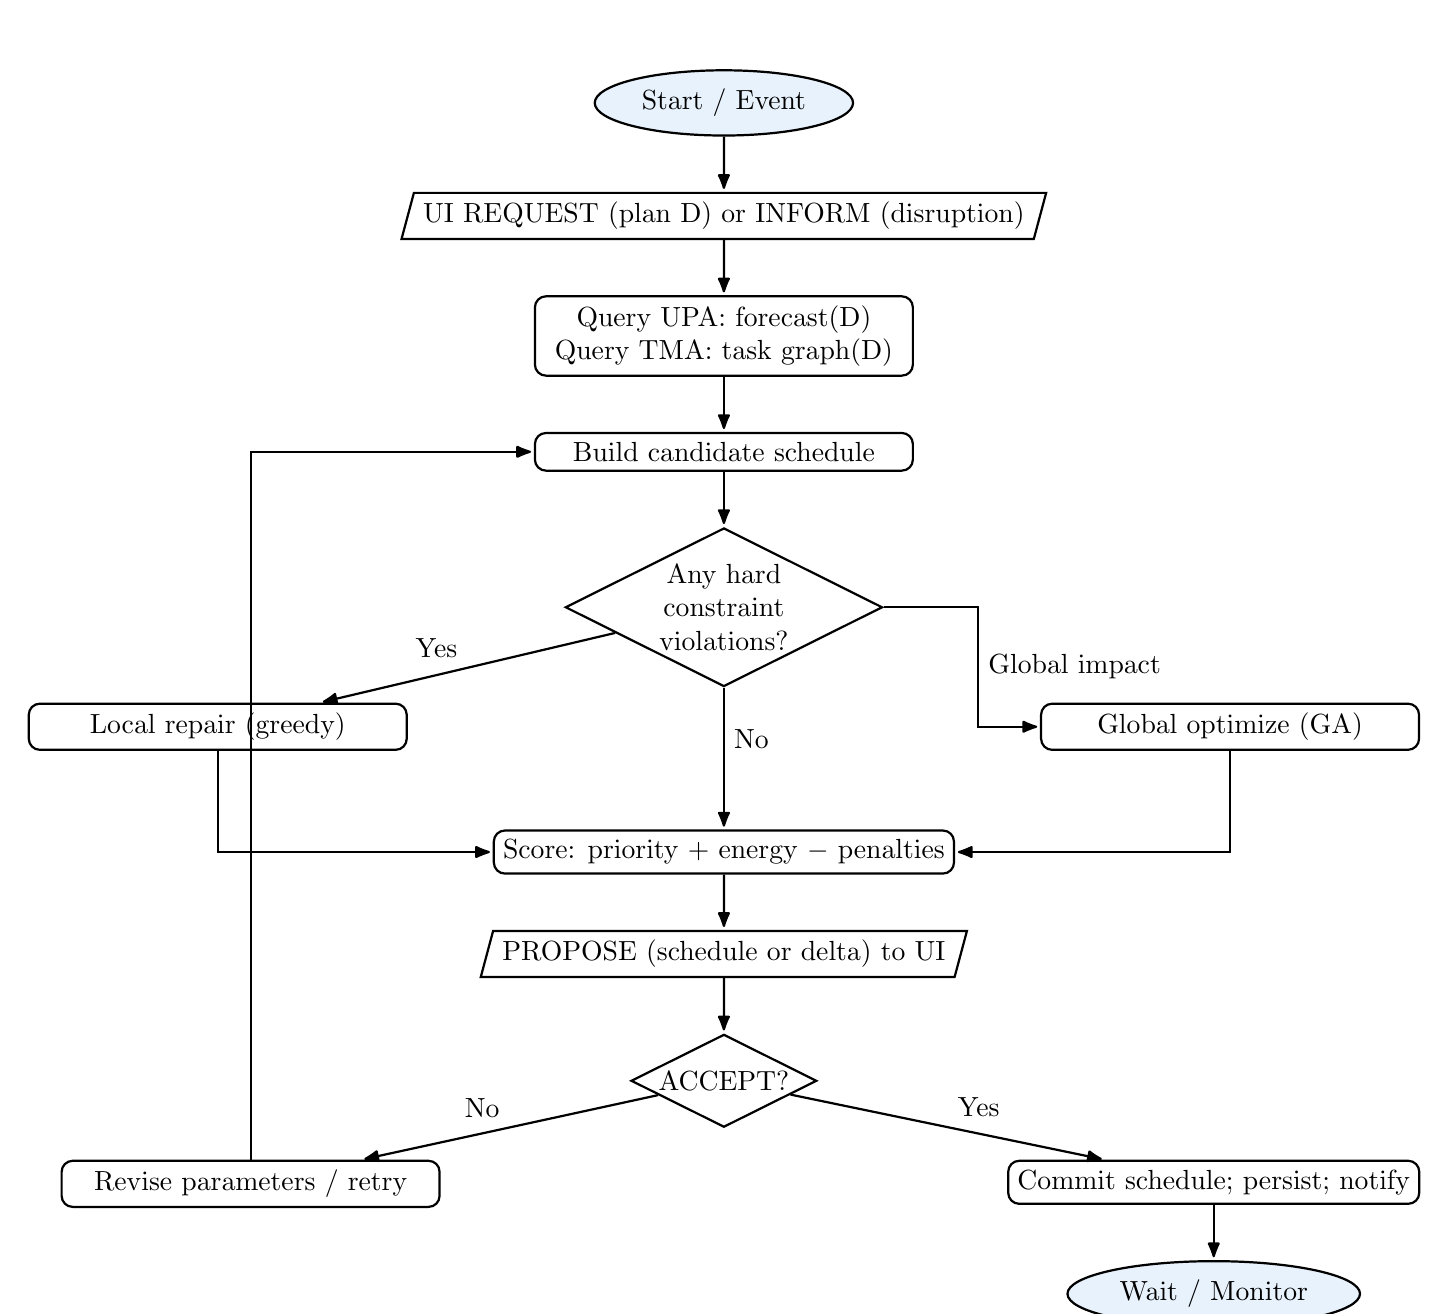
\begin{tikzpicture}[
  node distance=7mm and 12mm,
  startstop/.style={ellipse, draw, thick, fill=ABSELight, minimum width=2.8cm},
  process/.style={rectangle, draw, thick, rounded corners, fill=white, minimum width=4.8cm, align=center},
  decision/.style={diamond, draw, thick, aspect=2, fill=white, inner sep=1pt, align=center},
  io/.style={trapezium, trapezium left angle=75, trapezium right angle=105, draw, thick, fill=white, minimum width=4.8cm, align=center},
  arrow/.style={-{Latex[round]}, thick},
  >={Latex[round]}, shorten >=1pt
]
\node[startstop] (S) {Start / Event};
\node[io, below=of S] (req) {UI REQUEST (plan D) or INFORM (disruption)};
\node[process, below=of req] (gather) {Query UPA: forecast(D)\\Query TMA: task graph(D)};
\node[process, below=of gather] (candidate) {Build candidate schedule};
\node[decision, below=of candidate] (viol) {Any hard\\constraint\\violations?};
\node[process, below left=of viol, xshift=-18mm] (repair) {Local repair (greedy)};
\node[process, below right=of viol, xshift=18mm] (ga) {Global optimize (GA)};
\node[process, below=18mm of viol] (score) {Score: priority + energy $-$ penalties};
\node[io, below=of score] (prop) {PROPOSE (schedule or delta) to UI};
\node[decision, below=of prop] (acc) {ACCEPT?};
\node[process, below left=of acc, xshift=-18mm] (revise) {Revise parameters / retry};
\node[process, below right=of acc, xshift=18mm] (commit) {Commit schedule; persist; notify};
\node[startstop, below=of commit] (end) {Wait / Monitor};

\draw[arrow] (S) -- (req);
\draw[arrow] (req) -- (gather);
\draw[arrow] (gather) -- (candidate);
\draw[arrow] (candidate) -- (viol);
\draw[arrow] (viol) -- node[above left]{Yes} (repair);
\draw[arrow] (viol) -- node[above right]{No} (score);
\draw[arrow] (repair) |- (score);
\draw[arrow] (viol.east) -- ++(1.2,0) |- node[pos=0.25,right]{Global impact} (ga);
\draw[arrow] (ga) |- (score);
\draw[arrow] (score) -- (prop);
\draw[arrow] (prop) -- (acc);
\draw[arrow] (acc) -- node[above left]{No} (revise);
\draw[arrow] (revise) |- (candidate);
\draw[arrow] (acc) -- node[above right]{Yes} (commit);
\draw[arrow] (commit) -- (end);
\end{tikzpicture}
\end{adjustbox}
\caption{PAA planning and re-planning flow.}
\label{fig:paa-flow}
\end{figure}

\section{PAA Statechart}
\begin{figure}[h]
\centering
\includegraphics[width=1\textwidth]{paa-behavioural-statechart.png}
\caption{PAA behavioural statechart.}
\label{fig:paa-state}
\end{figure}


\section{Agent Workflow (End-to-End)}
\begin{figure}[h]
\centering

\caption{Agent workflow from task intake to plan commit.}
\label{fig:agent-workflow}
\end{figure}

\section{Fitness Function \& Local Repair}
\subsection*{Fitness Components}
\begin{tabularx}{\textwidth}{@{}p{3.6cm}p{3.2cm}X@{}}
\toprule
\textbf{Component} & \textbf{Weight Range} & \textbf{Notes} \\
\midrule
Priority Satisfaction & $w_p \in [0.3,0.6]$ & Task importance, deadlines, criticality path \\
Energy Alignment & $w_e \in [0.2,0.5]$ & Match energy curve to task difficulty \\
Travel/Transition Penalty & $w_t \in [0.0,0.2]$ & Minimize context switches/travel time \\
Constraint Penalty & $w_c \in [0.3,0.7]$ & Hard constraints get large negative penalties \\
\bottomrule
\end{tabularx}

\subsection*{Local Repair (pseudo-code)}
\begin{lstlisting}[style=code,caption={Greedy local repair at disruption}]
def local_repair(schedule, disruption):
    impacted = find_impacted_blocks(schedule, disruption)
    for block in sort_by_urgency(impacted):
        slots = enumerate_feasible_slots(schedule, block.task)
        best = argmax(slots, key=lambda s: score_delta(schedule, block, s))
        if best and respects_hard_constraints(best):
            schedule = place(schedule, block, best)
        else:
            return escalate_to_global(schedule, impacted)
    return schedule
\end{lstlisting}

%=============================
\chapter{Services Model}
%=============================
\begin{longtable}{@{}p{3.2cm}p{3.2cm}p{4.2cm}p{4.2cm}@{}}
\toprule
\textbf{Service} & \textbf{Inputs} & \textbf{Pre-Conditions} & \textbf{Post-Conditions / Failure Modes} \\
\midrule
GeneratePlan & task\_graph, energy\_forecast, availability & Valid DAG; availability defined & Schedule persisted; conflicts=0. Fail: invalid graph, timeout. \\
RePlanFast & disruption\_event & Current schedule exists & Delta applied; churn $\le \theta$. Fail: escalate to GA. \\
GlobalOptimize & task\_graph, energy\_forecast & Impact is global & New schedule proposed. Fail: timeout $\Rightarrow$ fallback template. \\
LearnPreferences & events, feedback & Data window available & Updated weights; monotonic constraints enforced. \\
\bottomrule
\end{longtable}

%=============================
\chapter{Data Specification}
%=============================
\section{Data Dictionary}
\begin{longtable}{@{}p{3.2cm}p{8.6cm}p{2.0cm}@{}}
\toprule
\textbf{Entity} & \textbf{Fields} & \textbf{Key} \\
\midrule
Task & id, title, deadline, effort, priority, status, depends\_on (nullable) & pk:id \\
ScheduleBlock & id, task\_id, start, end, confidence & pk:id, fk:task\_id \\
Preference & id, key, value (float), updated\_at & pk:id \\
Event & id, ts, type, payload(json) & pk:id \\
\bottomrule
\end{longtable}

\section{E--R Sketch}
\begin{figure}[h]
\centering
\begin{adjustbox}{max totalsize={\textwidth}{0.85\textheight},center}
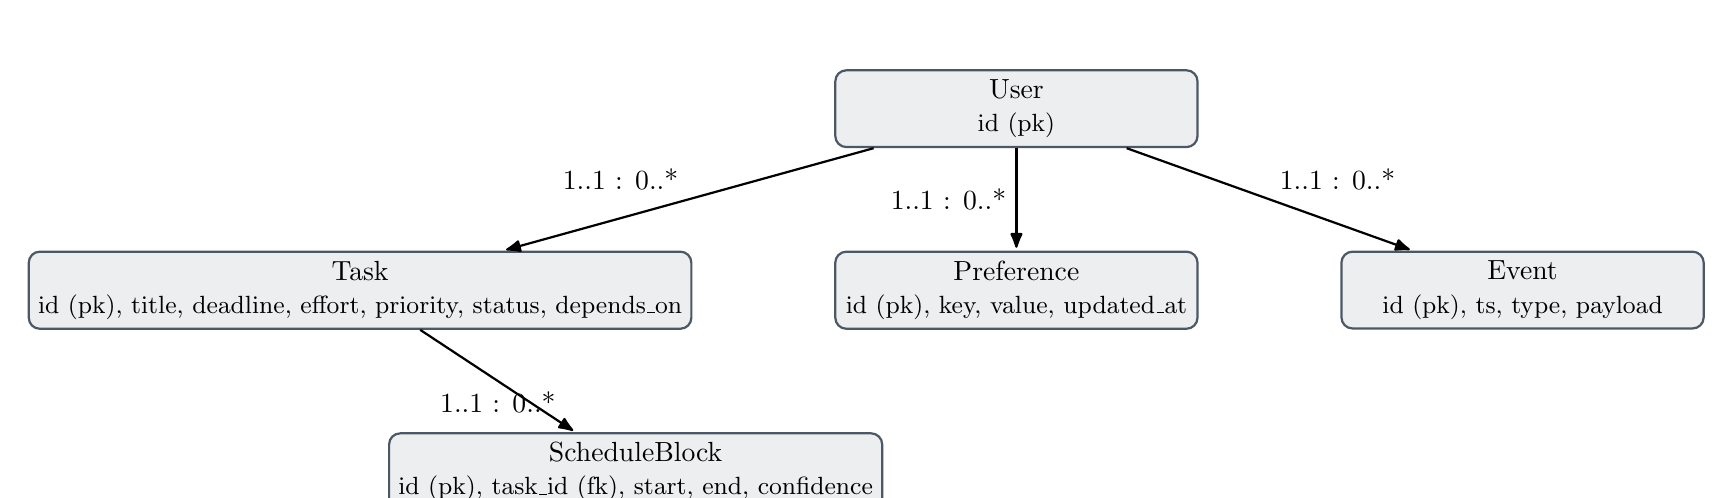
\begin{tikzpicture}[
  node distance=13mm and 18mm,
  entity/.style={rectangle, draw=ABSEGray, thick, rounded corners, minimum width=4.6cm, align=center, fill=ABSEGray!10},
  >={Latex[round]}, shorten >=1pt
]
\node[entity] (User){User\\\small id (pk)};
\node[entity, below left=of User] (Task){Task\\\small id (pk), title, deadline, effort, priority, status, depends\_on};
\node[entity, below=of User] (Pref){Preference\\\small id (pk), key, value, updated\_at};
\node[entity, below right=of User] (Event){Event\\\small id (pk), ts, type, payload};
\node[entity, below=of Task, xshift=35mm] (Block){ScheduleBlock\\\small id (pk), task\_id (fk), start, end, confidence};

\draw[->,thick] (User) -- node[midway,above left]{1..1 : 0..*} (Task);
\draw[->,thick] (User) -- node[midway,left]{1..1 : 0..*} (Pref);
\draw[->,thick] (User) -- node[midway,above right]{1..1 : 0..*} (Event);
\draw[->,thick] (Task) -- node[midway,below]{1..1 : 0..*} (Block);
\end{tikzpicture}
\end{adjustbox}
\caption{E--R sketch for MAPS storage.}
\label{fig:er}
\end{figure}

%=============================
\chapter{Quality Attributes \& Risks}
%=============================
\section{NFR Scenarios}
\begin{longtable}{@{}p{2.8cm}p{8.8cm}p{2.2cm}@{}}
\toprule
\textbf{Attribute} & \textbf{Scenario} & \textbf{Target} \\
\midrule
Performance & Initial plan for $\le 40$ tasks & $\le 2$s \\
Performance & Local re-plan after single overrun & p50 $\le 150$ms; p95 $\le 500$ms \\
Reliability & Crash during planning; on restart & Recover last committed schedule \\
Privacy & All data local; encrypted at rest & AES-256; minimal payloads over bus \\
\bottomrule
\end{longtable}

%=============================
\chapter{Acquaintance Model \& Summary}
%=============================
\section{Acquaintance Model}
UI $\leftrightarrow$ PAA (plan lifecycle), UI $\leftrightarrow$ TMA (task CRUD), UI $\leftrightarrow$ UPA (feedback), PAA $\leftrightarrow$ UPA (forecasts), PAA $\leftrightarrow$ TMA (graphs), All $\rightarrow$ Logger.

\section{Summary}
This extended GAIA design provides traceability from goals to roles and services, formalizes protocols and message schemas, details PAA behaviour via flowchart and statechart, and adds an end-to-end agent workflow for implementation (SPADE/JADE) and assessment.

\end{document}
